\begin{figure}
    \centering
    \begin{subfigure}{0.8\linewidth}
        \centering
        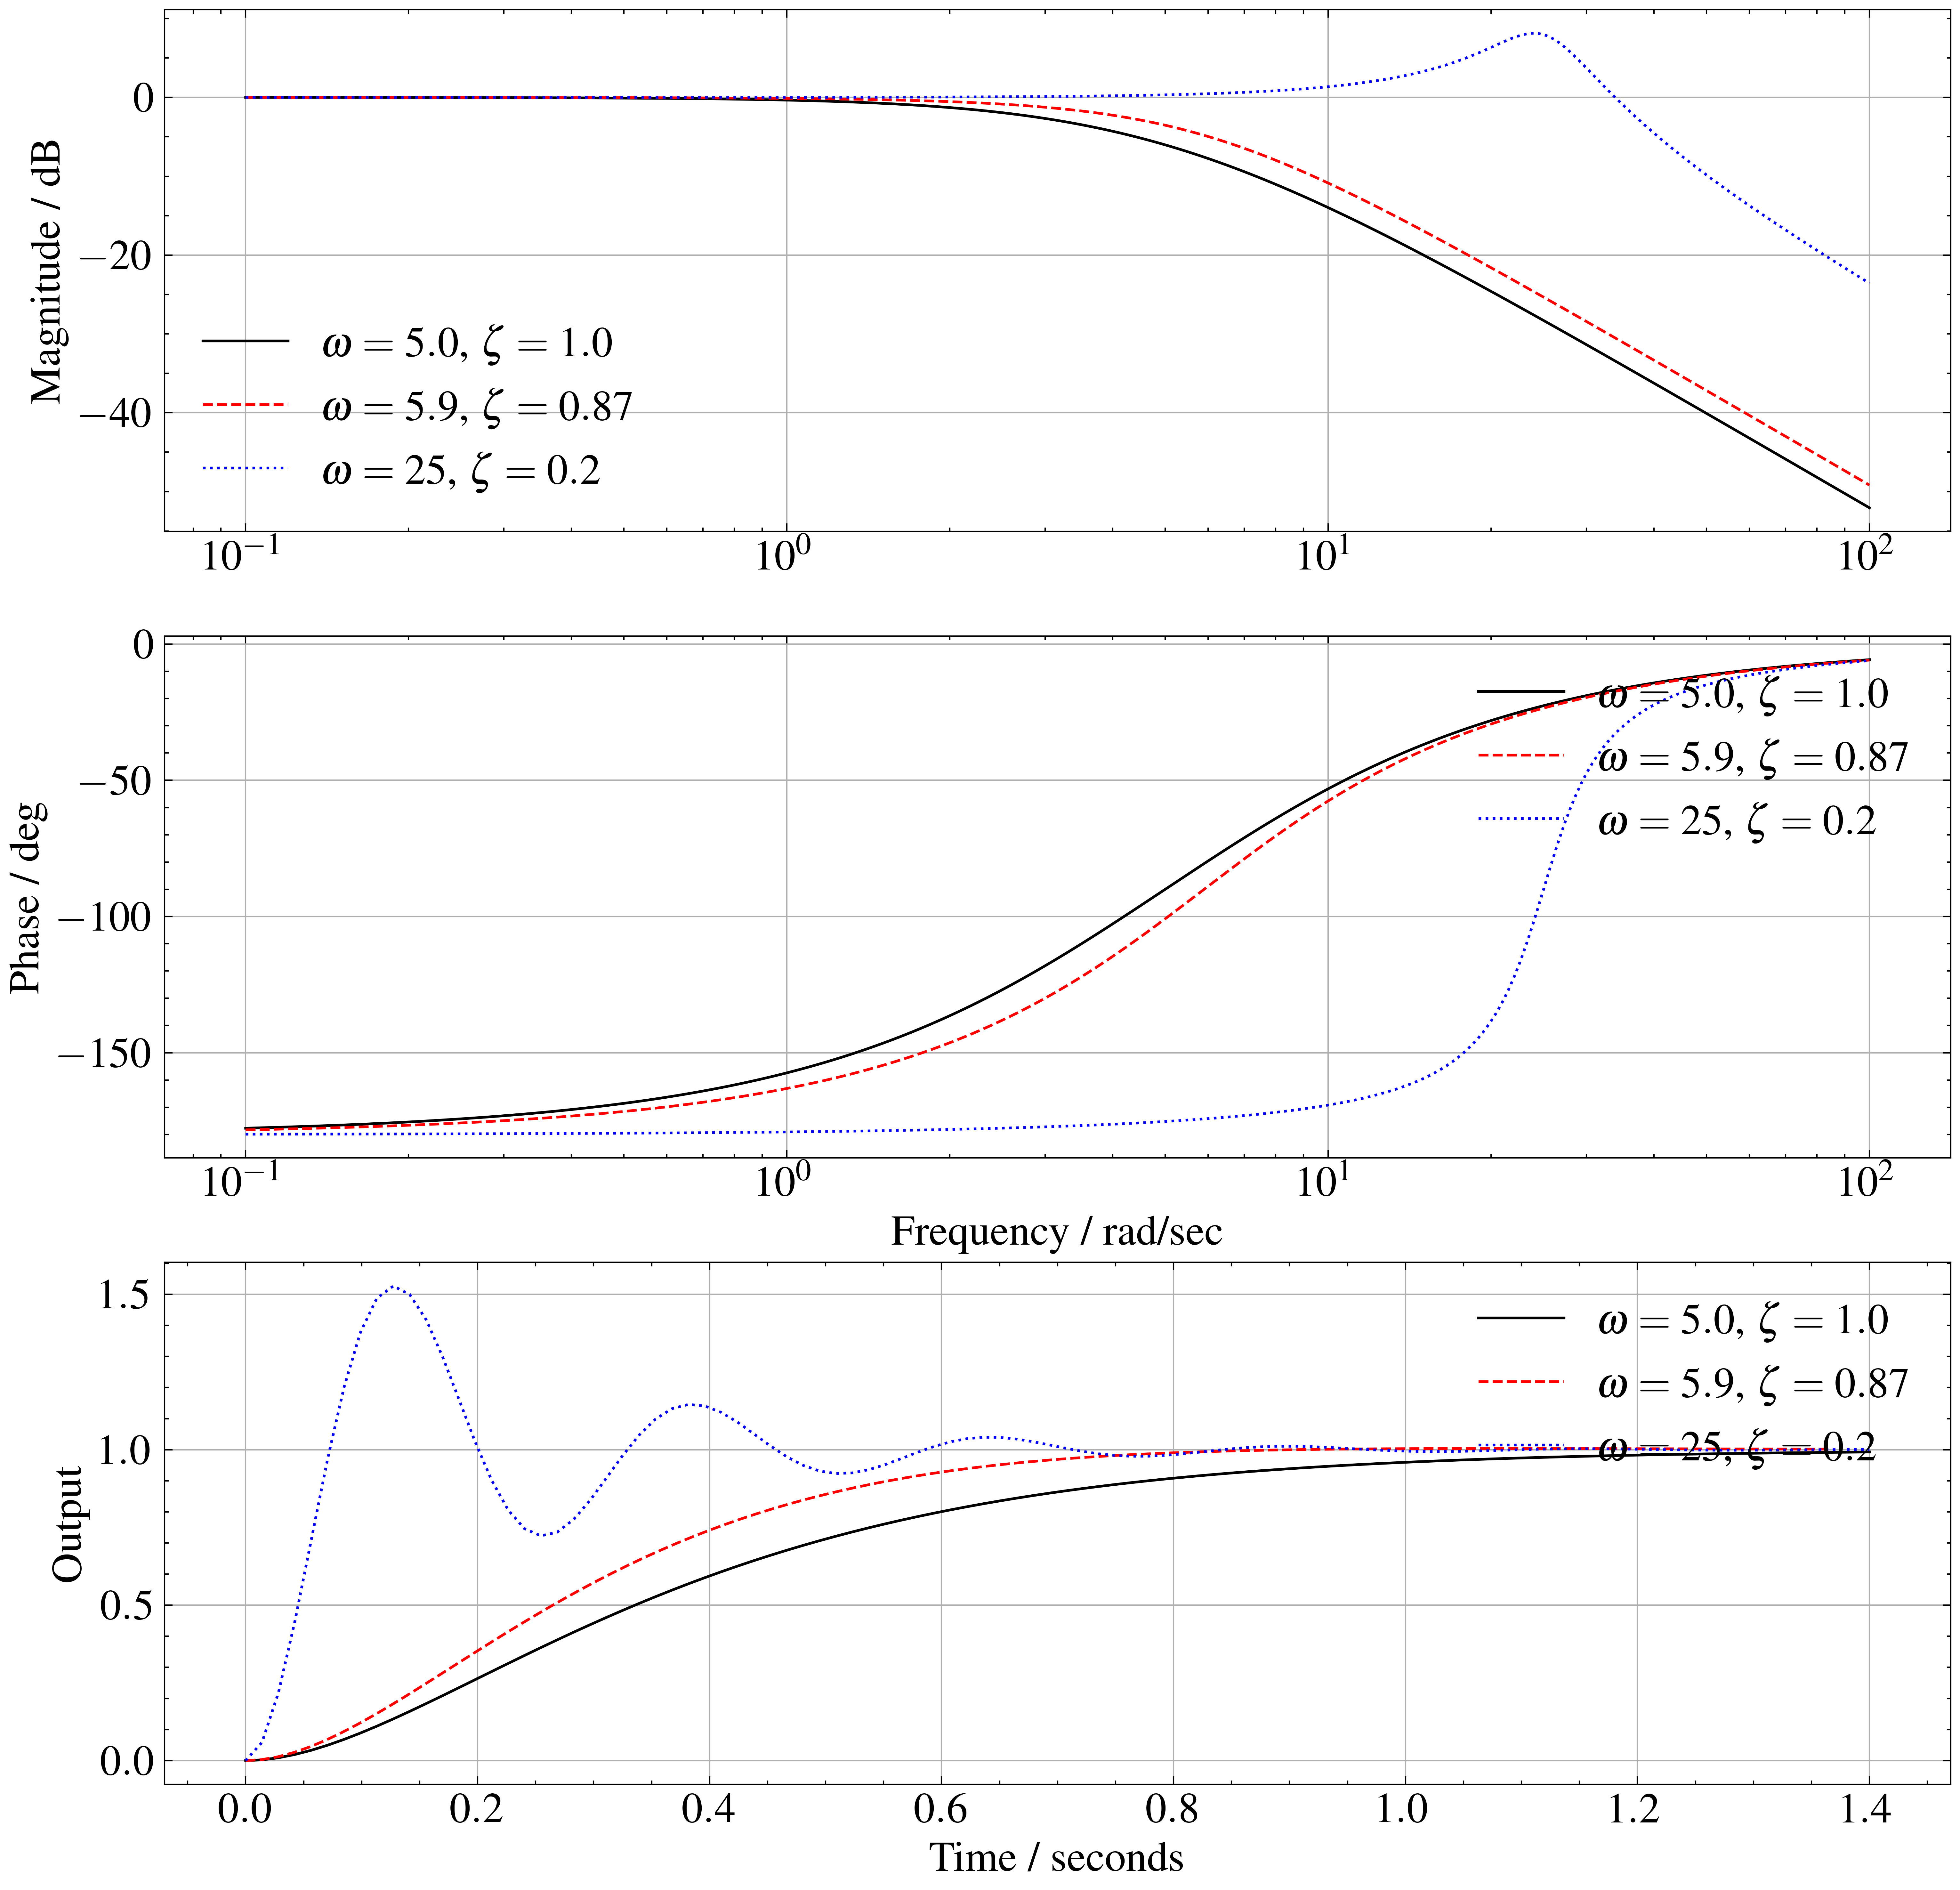
\includegraphics[width=0.8\linewidth]{src/figures/bode-phase-step-ideal-group-real/bode-phase-step-ideal-group-real-1.png}
        \subcaption{$D = 0$のときの$\zeta$、$\omega$の近侍値に対するボード線図とステップ応答}\label{fig:bode-phase-step-ideal-group-real-d-0}
    \end{subfigure}
    \begin{subfigure}{0.8\linewidth}
        \centering
        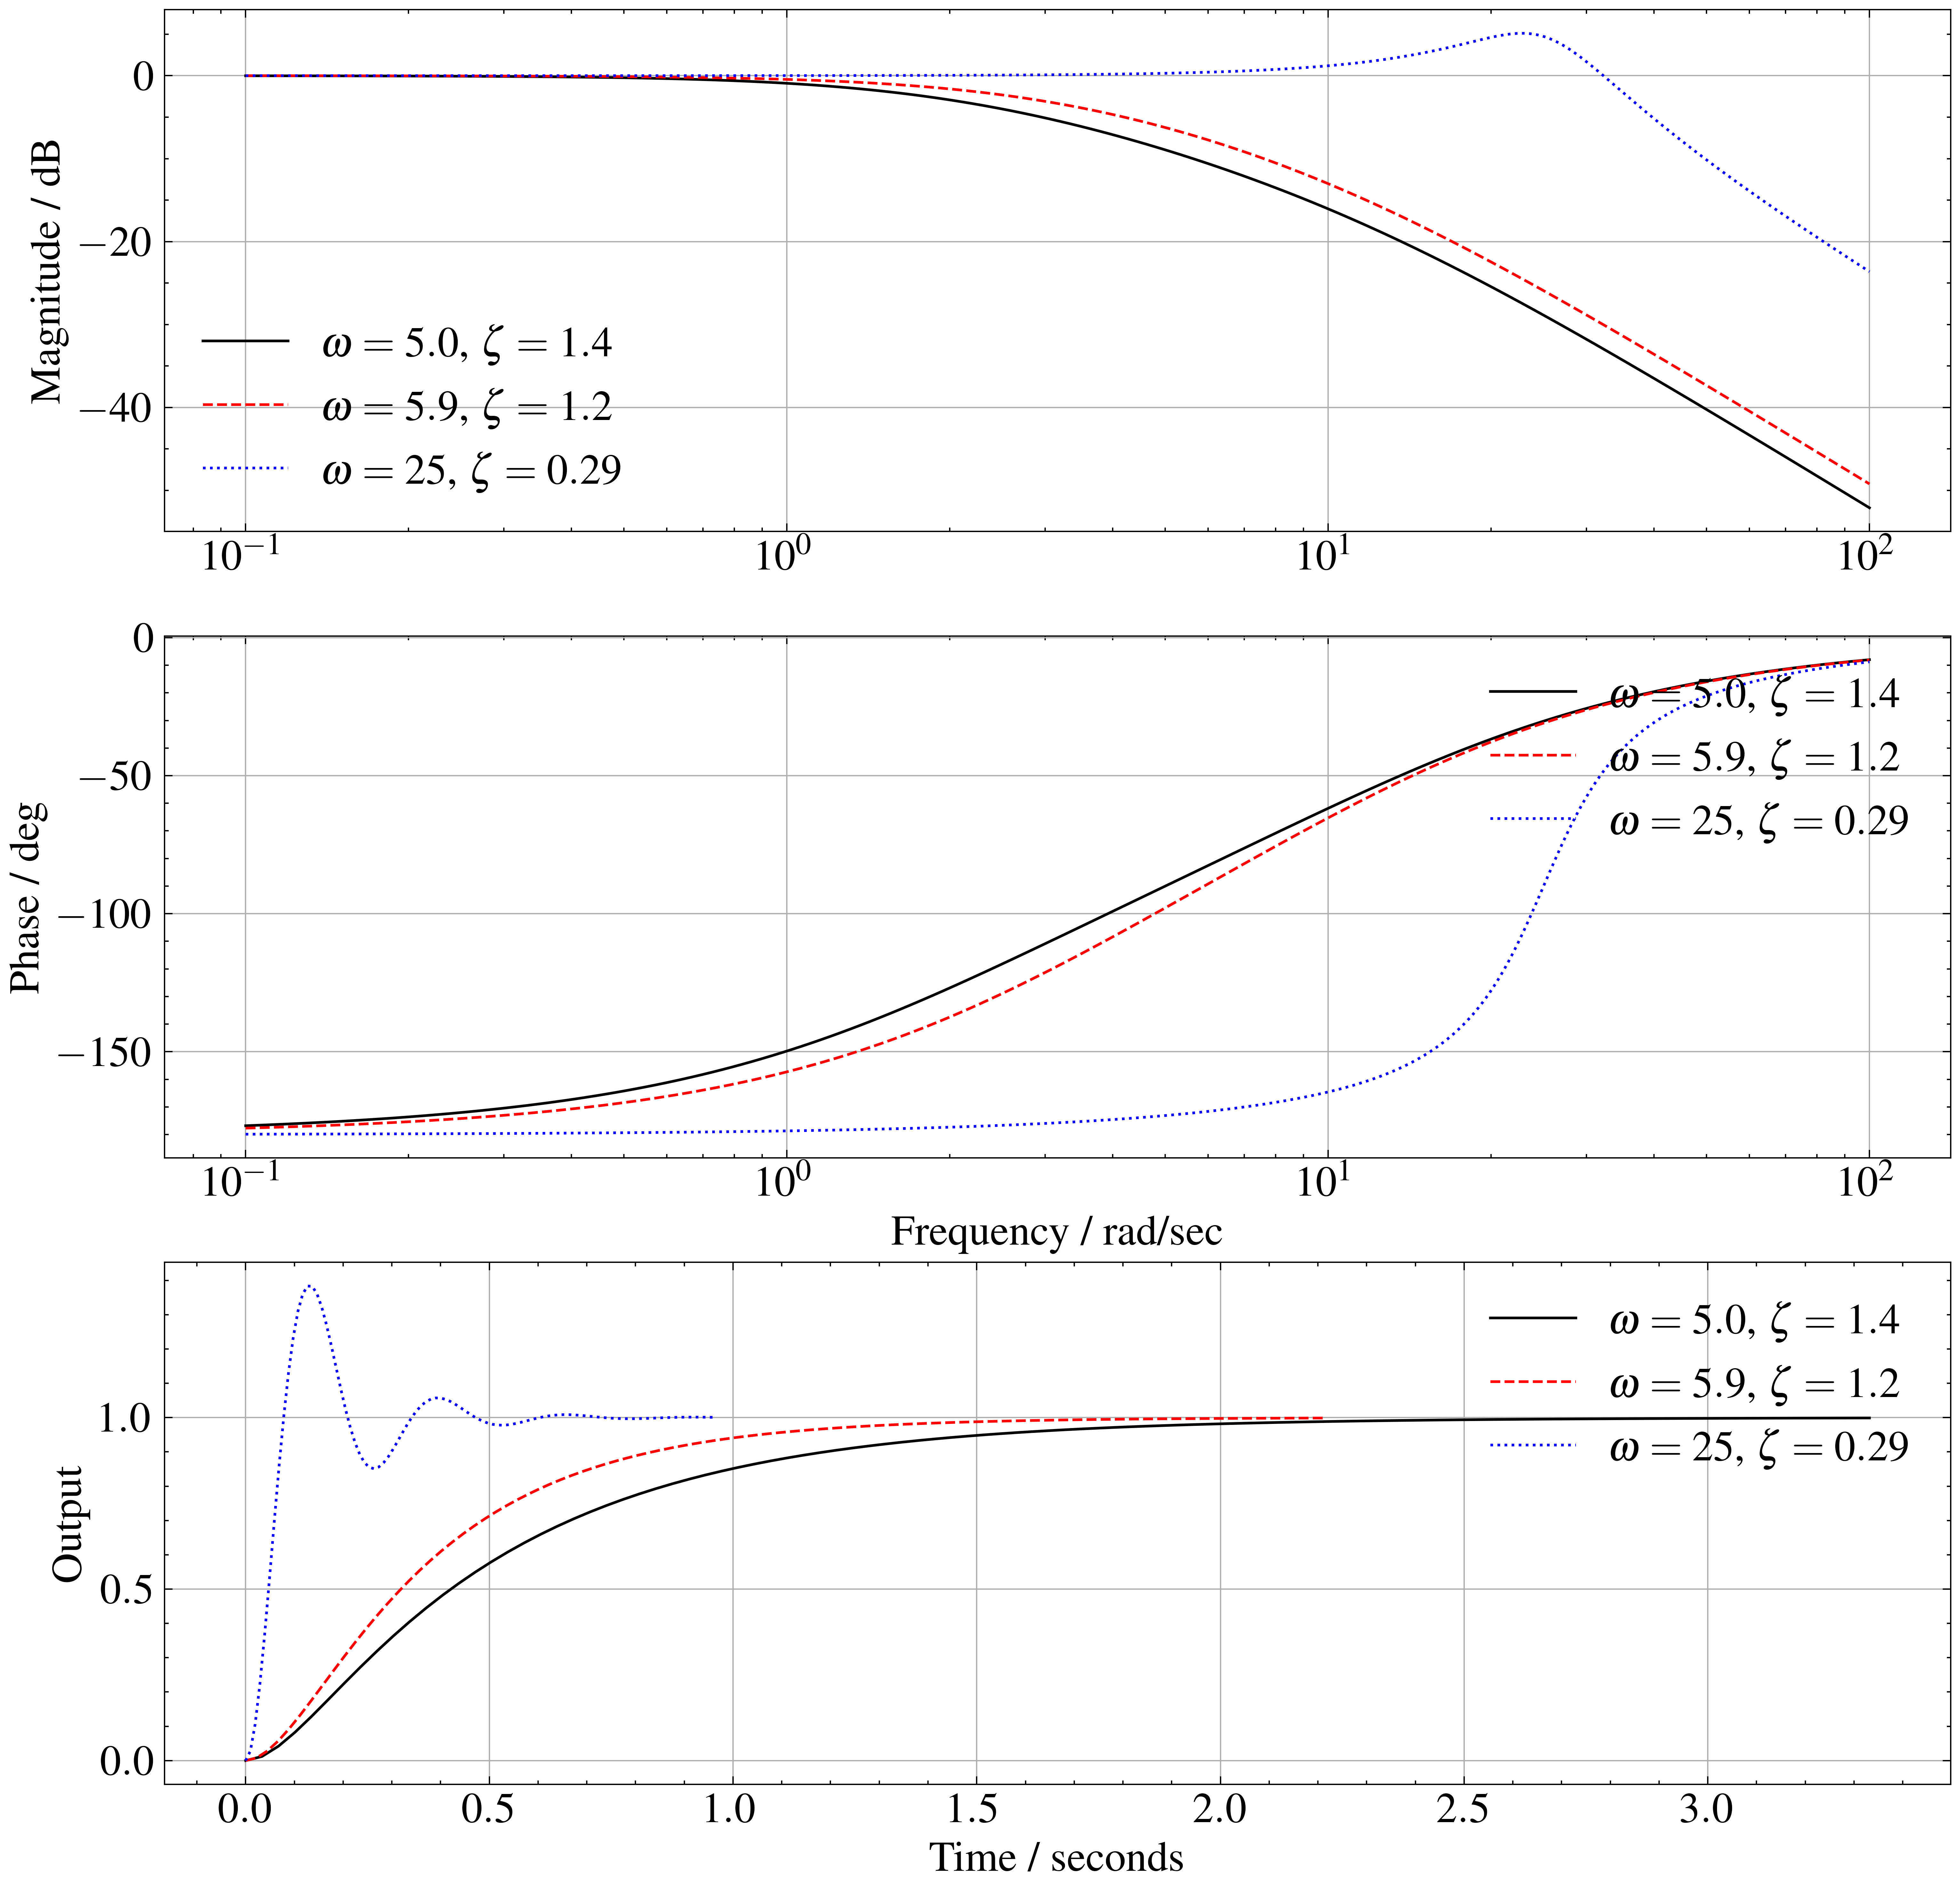
\includegraphics[width=0.8\linewidth]{src/figures/bode-phase-step-ideal-group-real/bode-phase-step-ideal-group-real-2.png}
        \subcaption{$D = 60$のときの$\zeta$、$\omega$の近侍値に対するボード線図とステップ応答}\label{fig:bode-phase-step-ideal-group-real-d-60}
    \end{subfigure}
    \caption{ある$D$に対して、$P$を変化させたときのボード線図とステップ応答}\label{fig:bode-phase-step-ideal-group-real}
\end{figure}


\begin{figure}
    \addtocounter{figure}{-1}
    \centering
    \begin{subfigure}{0.8\linewidth}
        \setcounter{subfigure}{2}
        \centering
        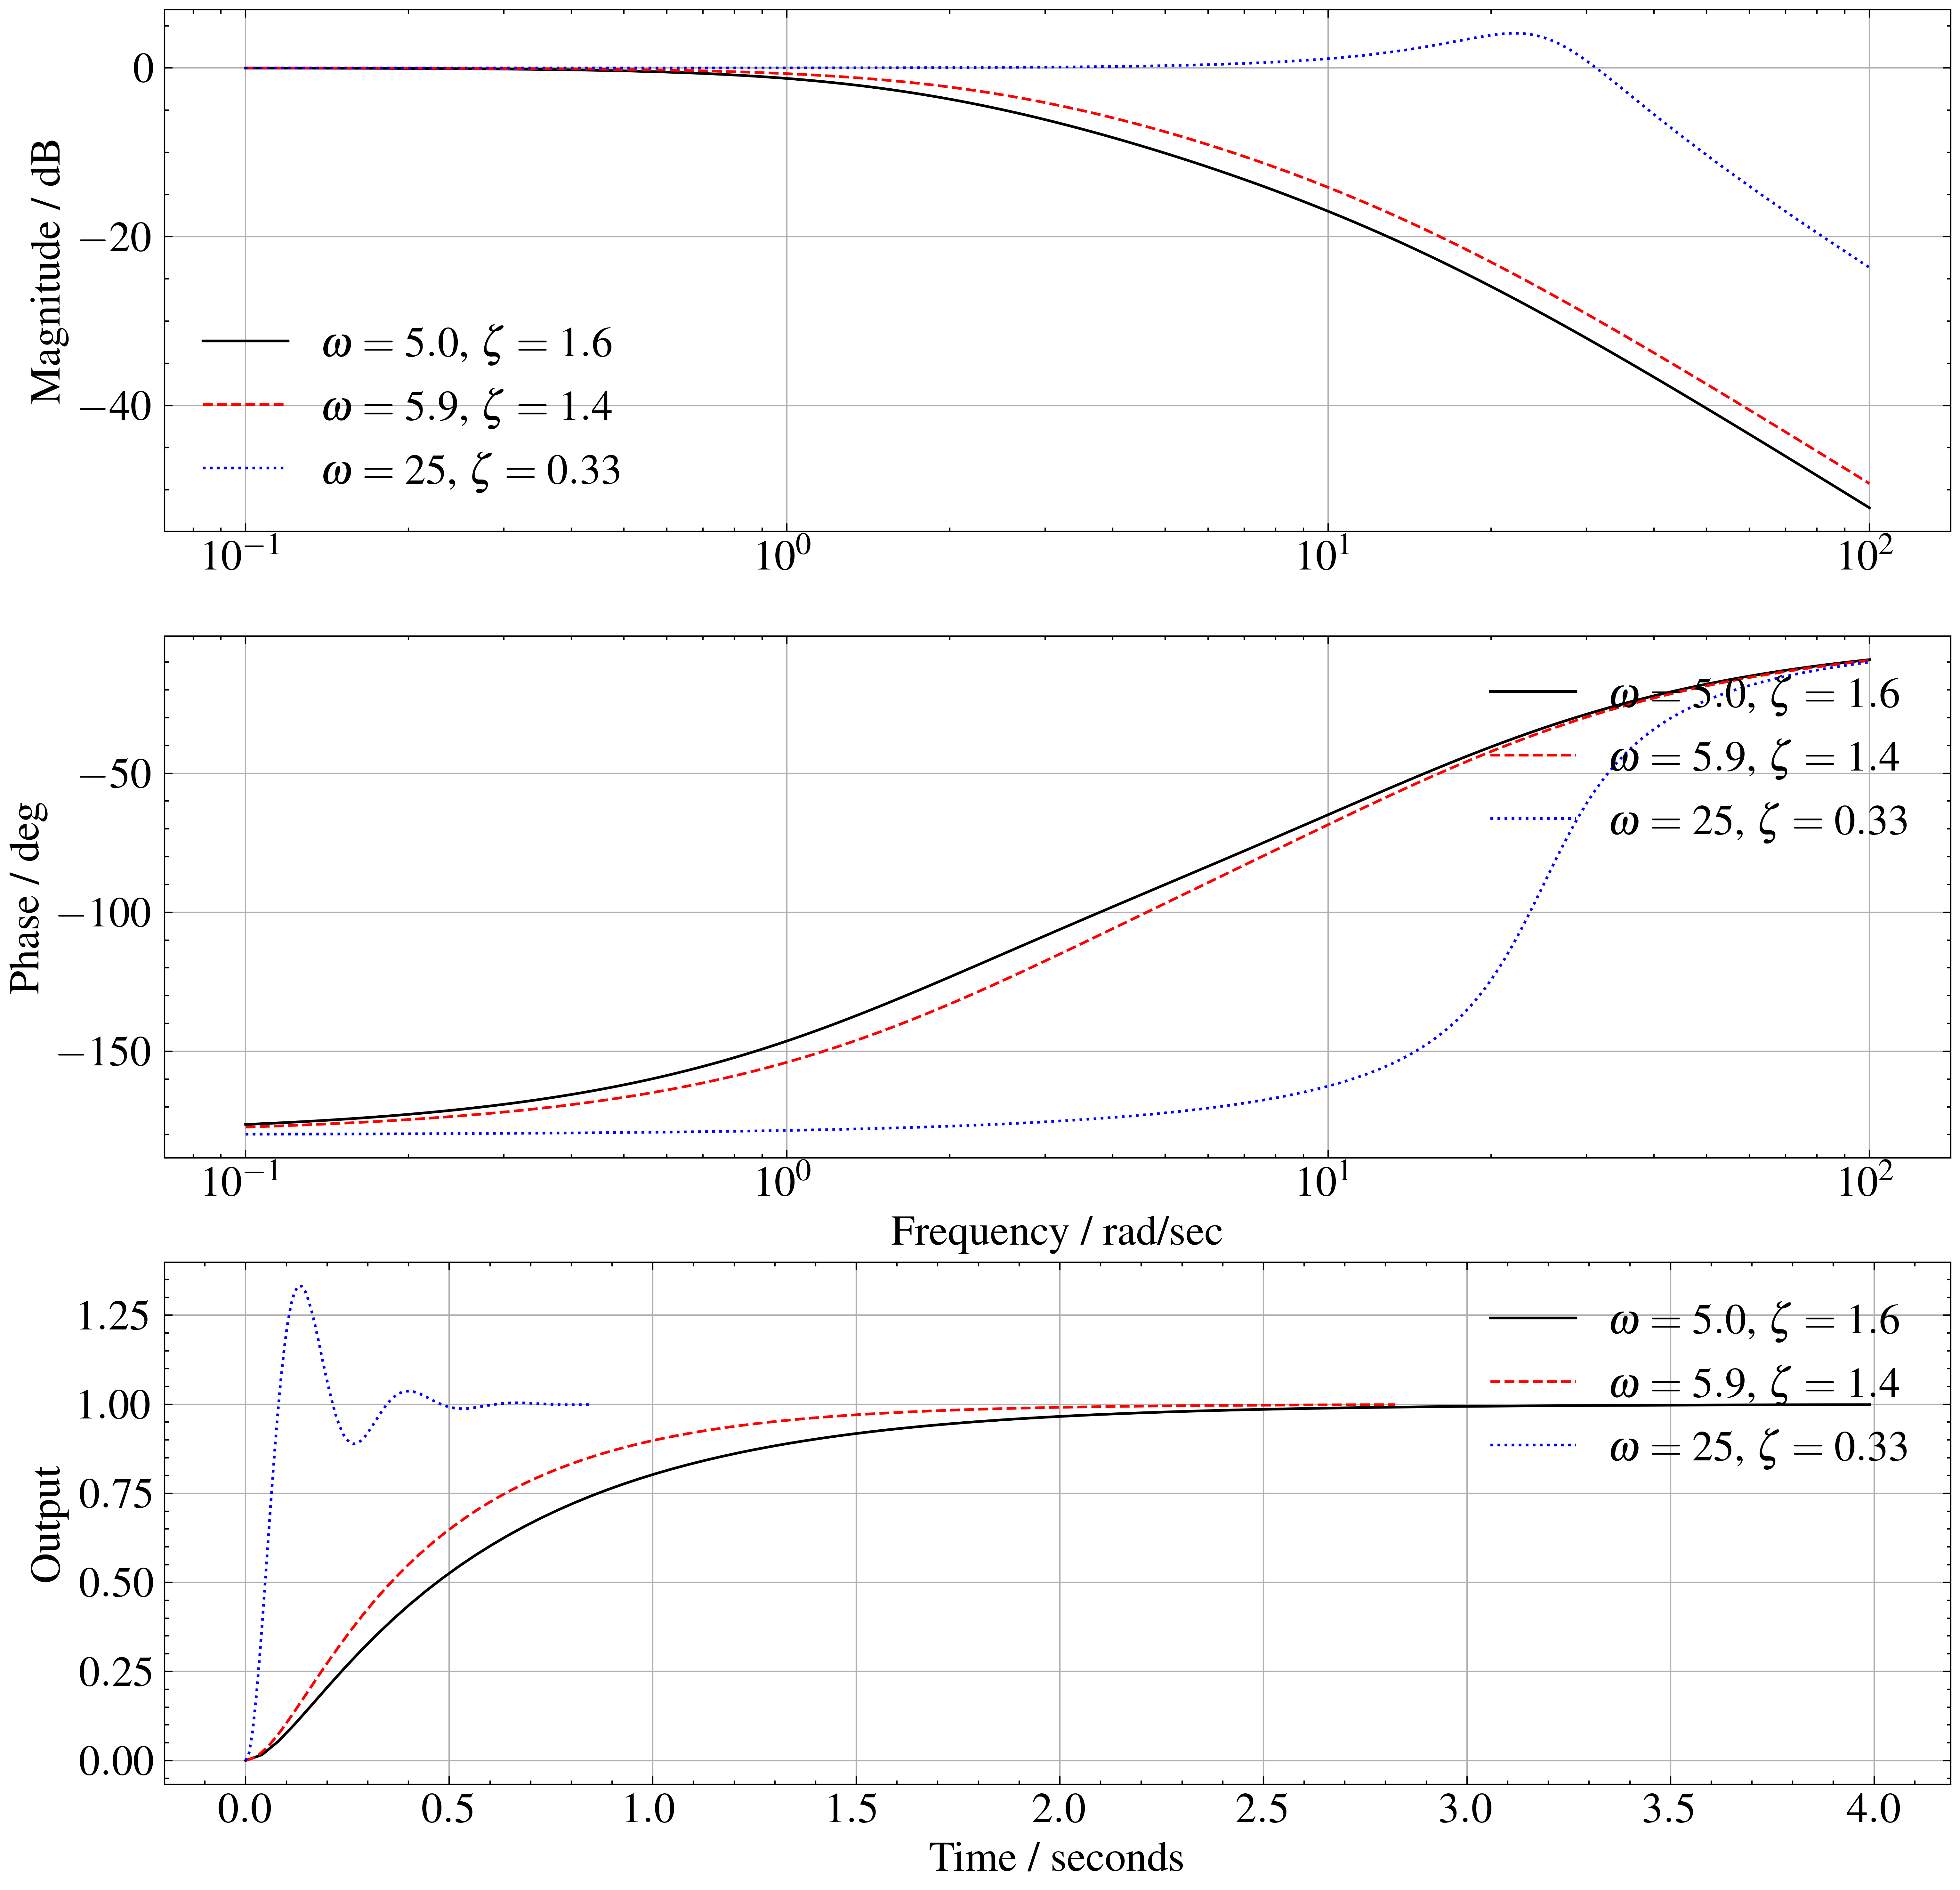
\includegraphics[width=0.8\linewidth]{src/figures/bode-phase-step-ideal-group-real/bode-phase-step-ideal-group-real-3.png}
        \subcaption{$D = 80$のときの$\zeta$、$\omega$の近侍値に対するボード線図とステップ応答}\label{fig:bode-phase-step-ideal-group-real-d-80}
    \end{subfigure}
    \begin{subfigure}{0.8\linewidth}
        \centering
        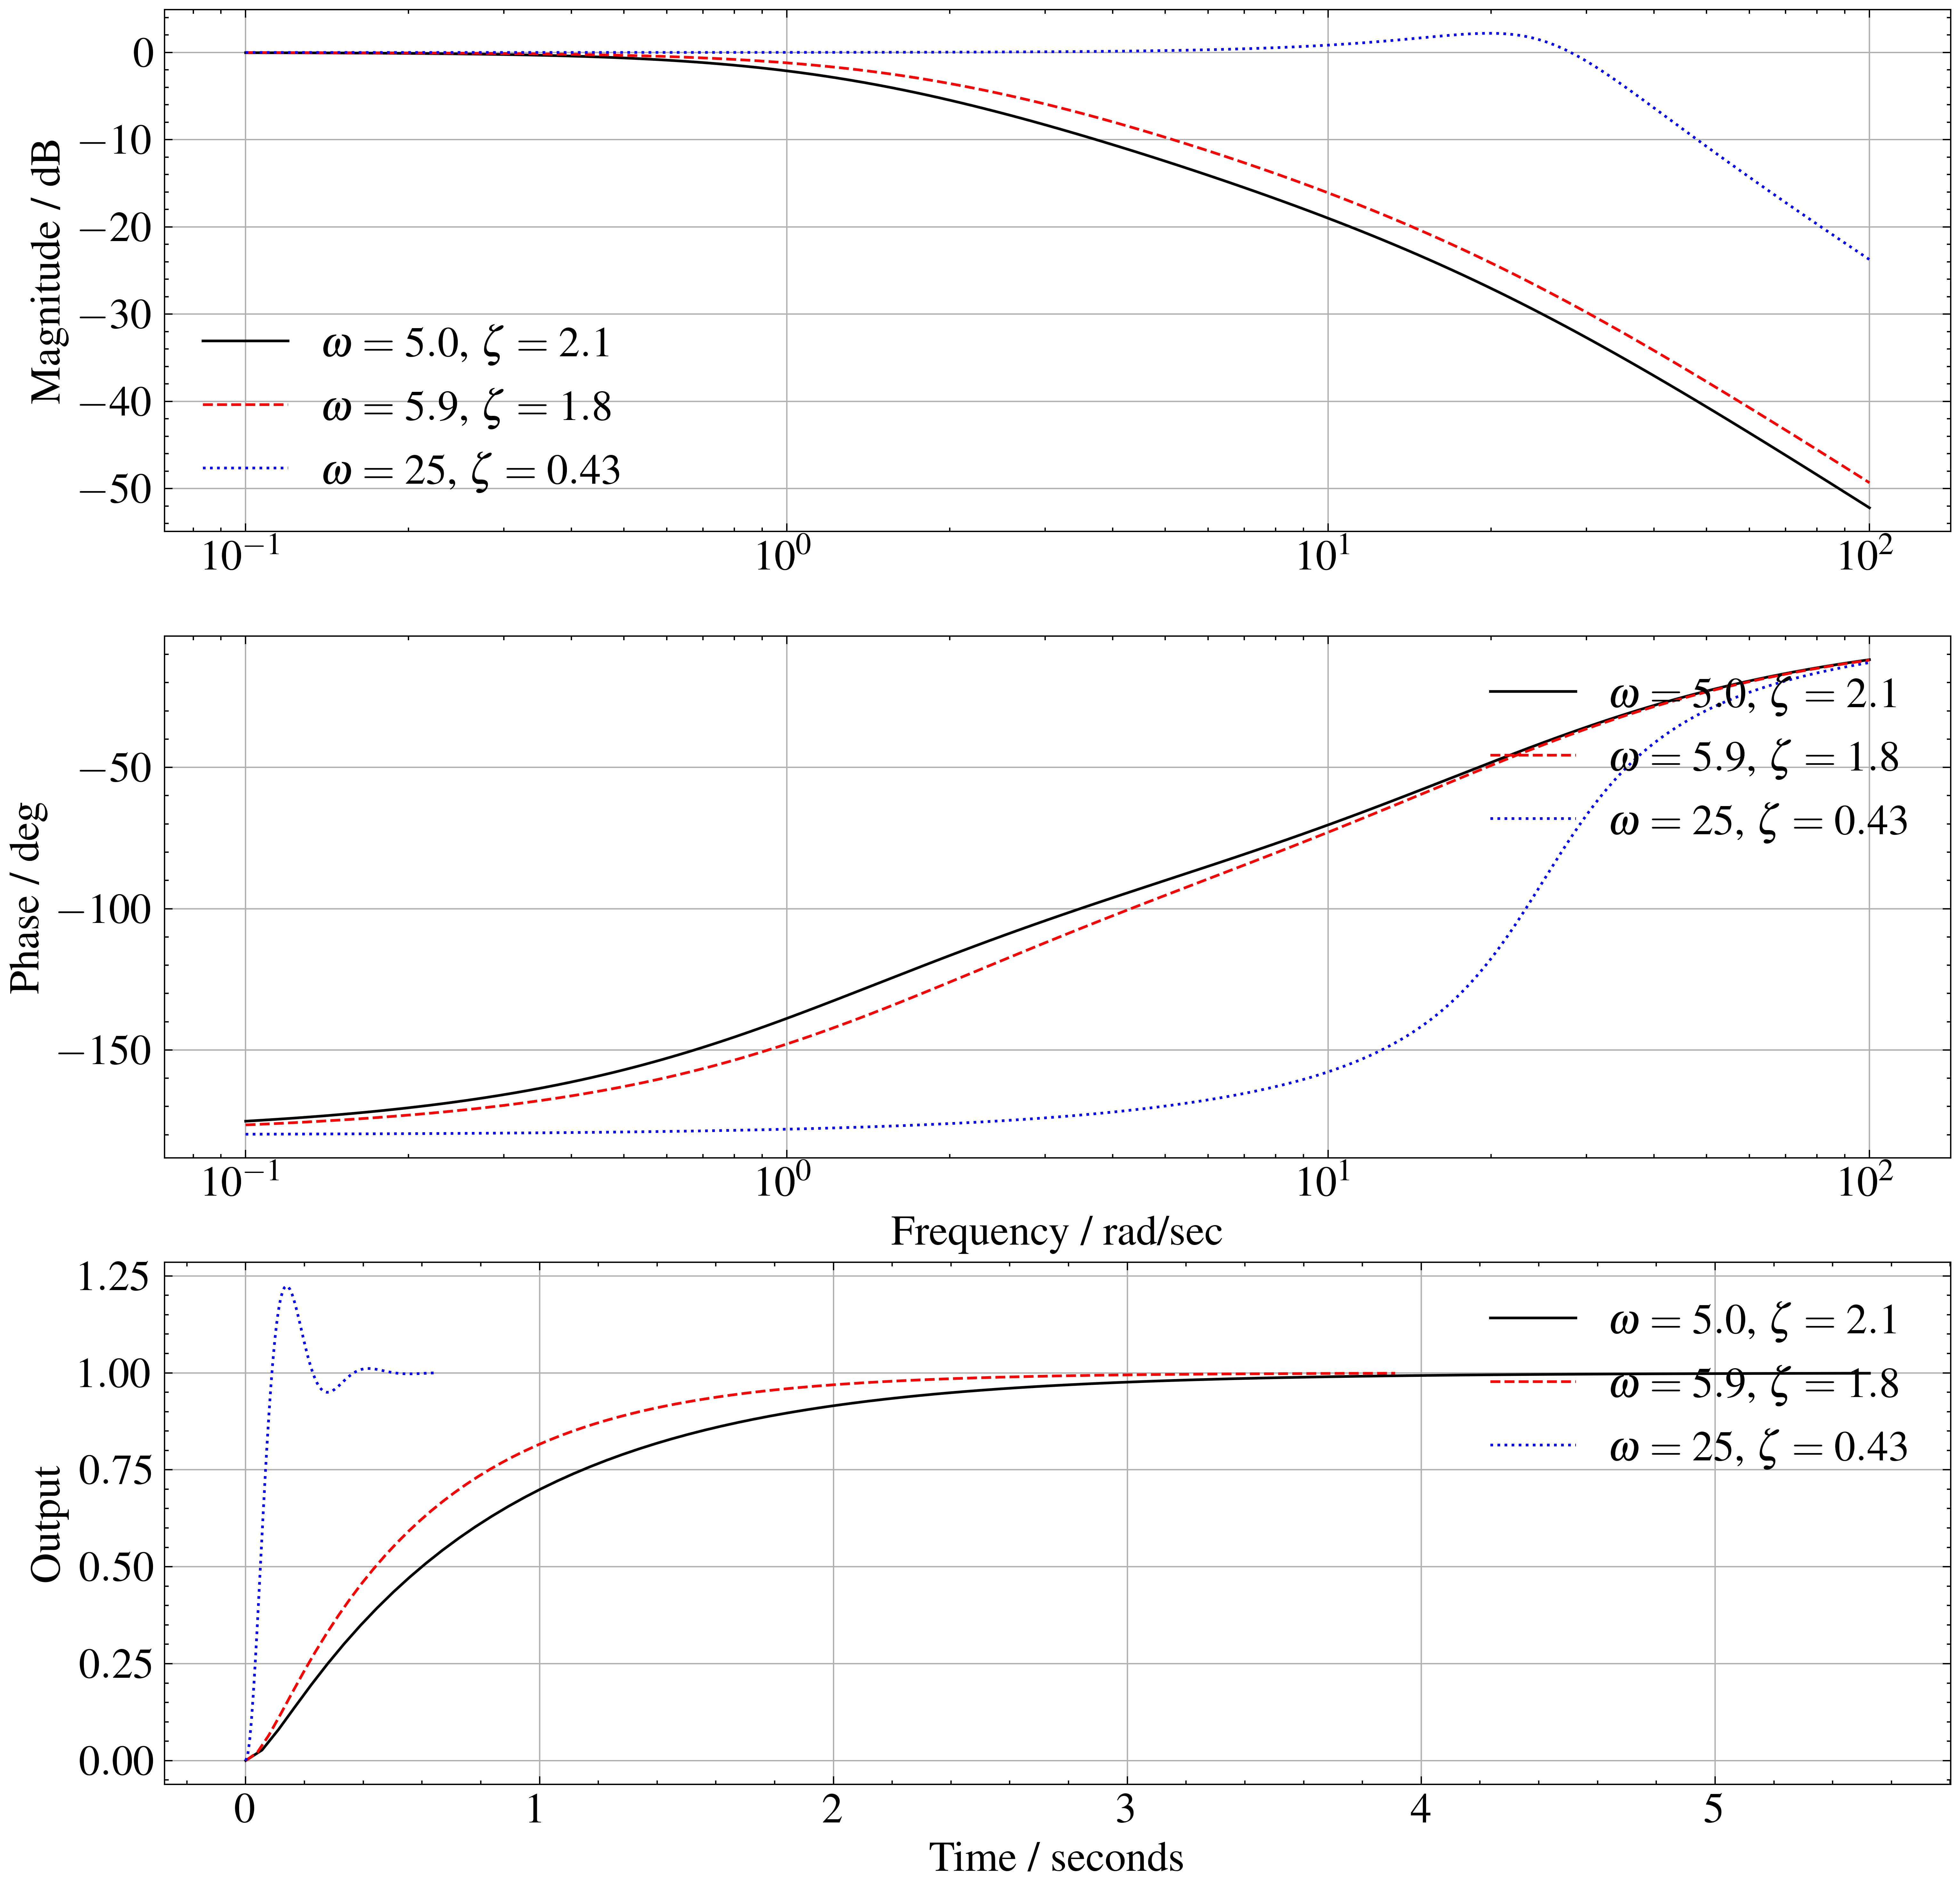
\includegraphics[width=0.8\linewidth]{src/figures/bode-phase-step-ideal-group-real/bode-phase-step-ideal-group-real-4.png}
        \subcaption{$D = 100$のときの$\zeta$、$\omega$の近侍値に対するボード線図とステップ応答}\label{fig:bode-phase-step-ideal-group-real-d-100}
    \end{subfigure}
    \caption{ある$D$に対して、$P$を変化させたときのボード線図とステップ応答(続き)}
\end{figure}
